\documentclass[a4paper,12pt]{article}
\newcounter{example}[]
\newenvironment{example}[1][]{\refstepcounter{example}\par\medskip
   \noindent \textbf{Example~\theexample. #1} \rmfamily}{\medskip}
   %%%%%%%%%%%%%%%%%%%%%%%%%%%%%%%%

%%%%%%%%%%%%%%%%%%%%%%%%%%%%%%%%%%
\usepackage[utf8]{inputenc}
\usepackage[english]{babel}
\usepackage{tikz-cd}
\usepackage{amsmath,amsfonts,amssymb,amsthm}
\usepackage{mathtools}
 \usepackage{float}
\usepackage{amsthm}
\usepackage{cite}
\usepackage{datetime} % British format dates
\usepackage[cm]{fullpage}
\usepackage{url}
\usepackage{hyperref}
\usepackage{stackrel,amssymb,amsmath}
\usepackage[nottoc]{tocbibind}
\usepackage{pgfplots}
\usepackage{rotating}
\usepackage[autostyle]{csquotes}
\usepackage{natbib}
\usepackage{graphicx}
\usepackage{natbib}
\usepackage{graphicx}

\newtheorem{problem}{Problem}
\newtheorem{attempt}{Attempt}


\newtheorem{theorem}{Theorem}[section]
\newtheorem{corollary}{Corollary}[theorem]
\newtheorem{lemma}[theorem]{Lemma}
\newtheorem{proposition}[theorem]{Proposition}
\theoremstyle{definition}
\newtheorem{definition}{Definition}[section]
\theoremstyle{indented}
\newtheorem*{remark}{Remark}
\newenvironment{titlemize}[1]{%
  \paragraph{#1}
  \begin{itemize}}
  {\end{itemize}}
  
  \usepackage[T1]{fontenc}
\usepackage{imakeidx}
\makeindex[columns=3, title=Alphabetical Index, intoc]
  
  
  %%%%%%%%%%5
\newcommand{\rightarrowdbl}{\rightarrow\mathrel{\mkern-14mu}\rightarrow}

\newcommand{\xrightarrowdbl}[2][]{%
  \xrightarrow[#1]{#2}\mathrel{\mkern-14mu}\rightarrow
}
%%%%%%%%%%%%%%5

\title{Leftovers}
\author{Rhys Wells}
\date{\today}

\begin{document}

\maketitle

\begin{titlemize} {Objectives}

\item 

\end{titlemize}


\begin{theorem}(Deletion-Restriction) Let $(\mathcal{A}, \mathcal{A^{'}},\mathcal{A^{''}} )$ be a triple of arrangements in $\mathbb{R}^n$. Then

$$\chi_{{\mathcal{A}}} (t) = \chi_{{\mathcal{A^{'}}}} (t) - \chi_{{\mathcal{A^{''}}}} (t)$$
\end{theorem}

\begin{figure}[H]
    \centering
 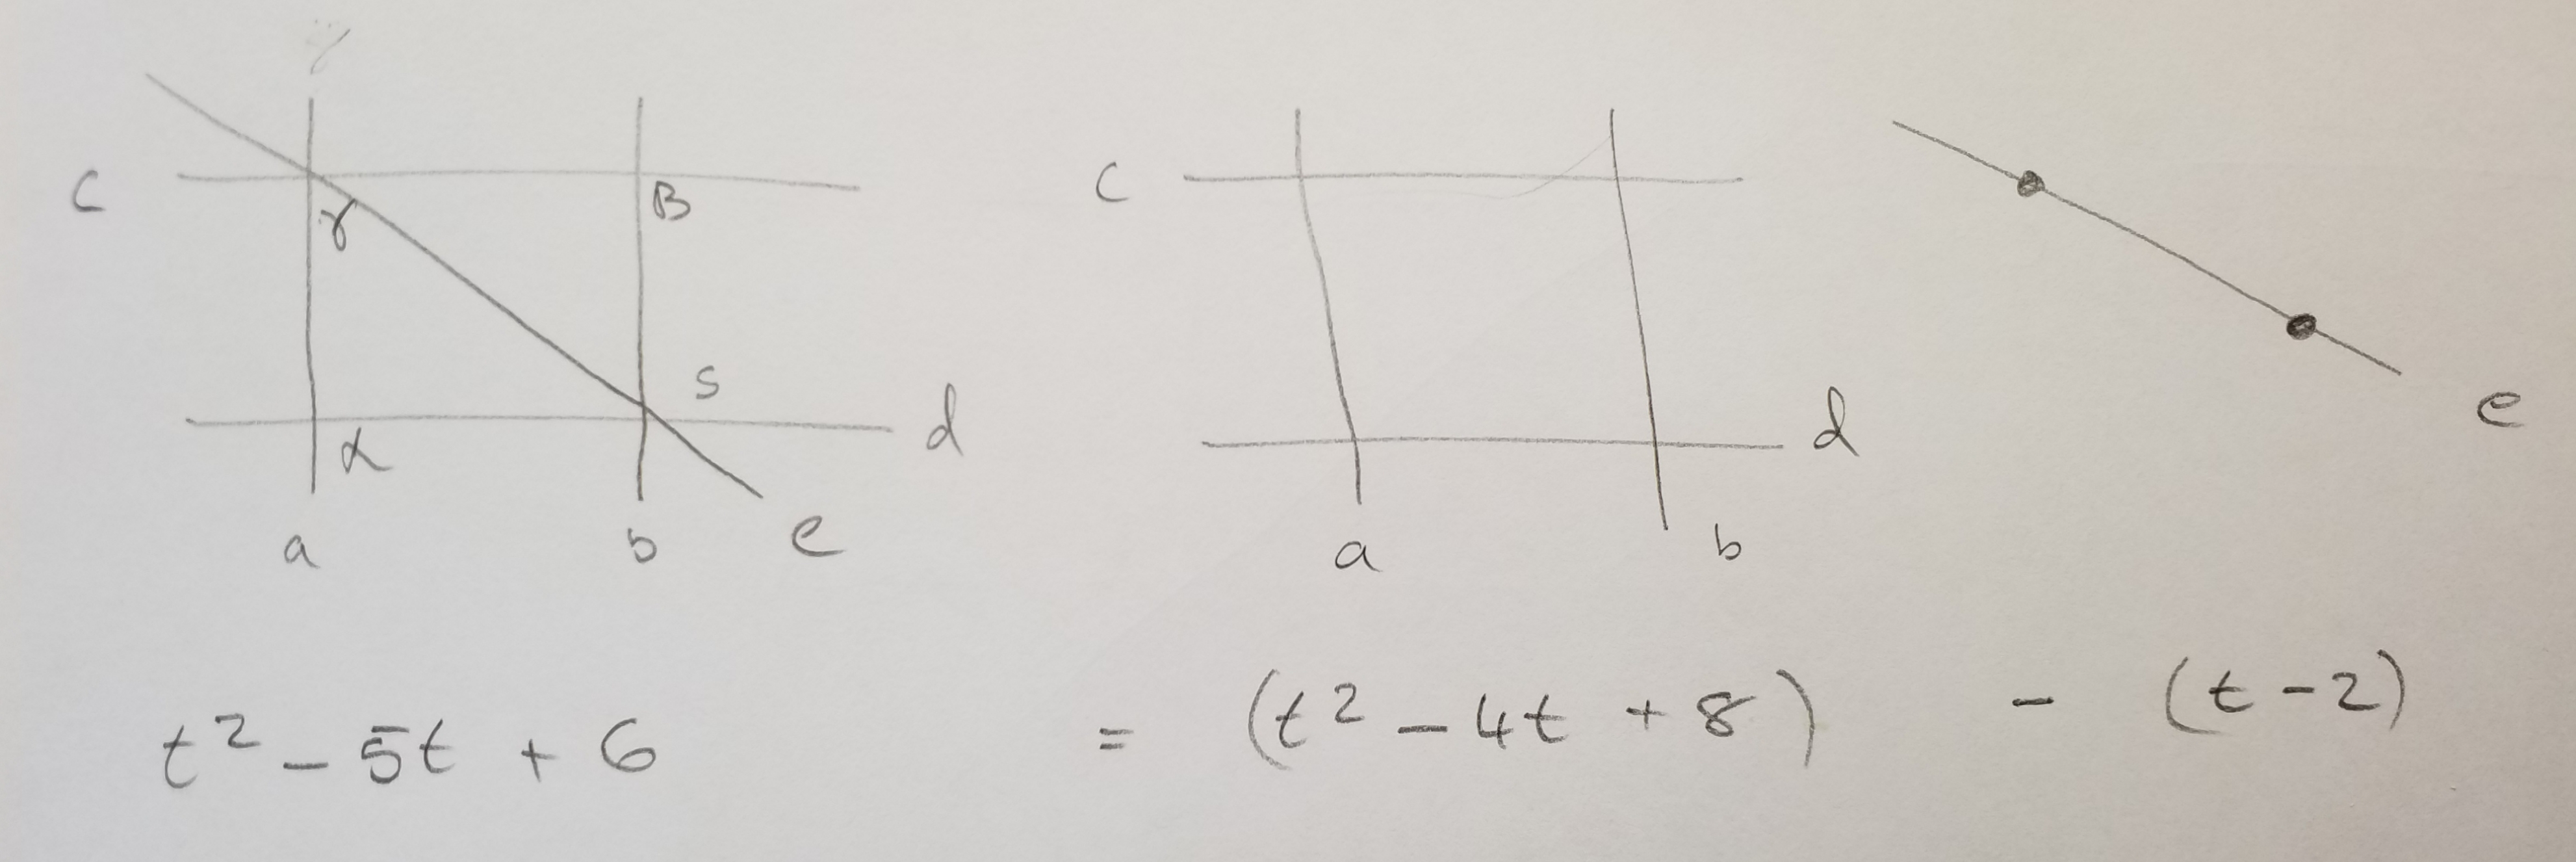
\includegraphics[scale=0.10,angle=0]{29072020 pics/del-res.jpg}  
    \caption{Deletion-restriction of Figure 1}
    \label{poset}
\end{figure}

\begin{titlemize}{Question}
\item How important is the choice in restriction to a particular $H$? Can we make solving our problem easier if we choose $H$ is a nice way. \begin{figure}[H]
    \centering
 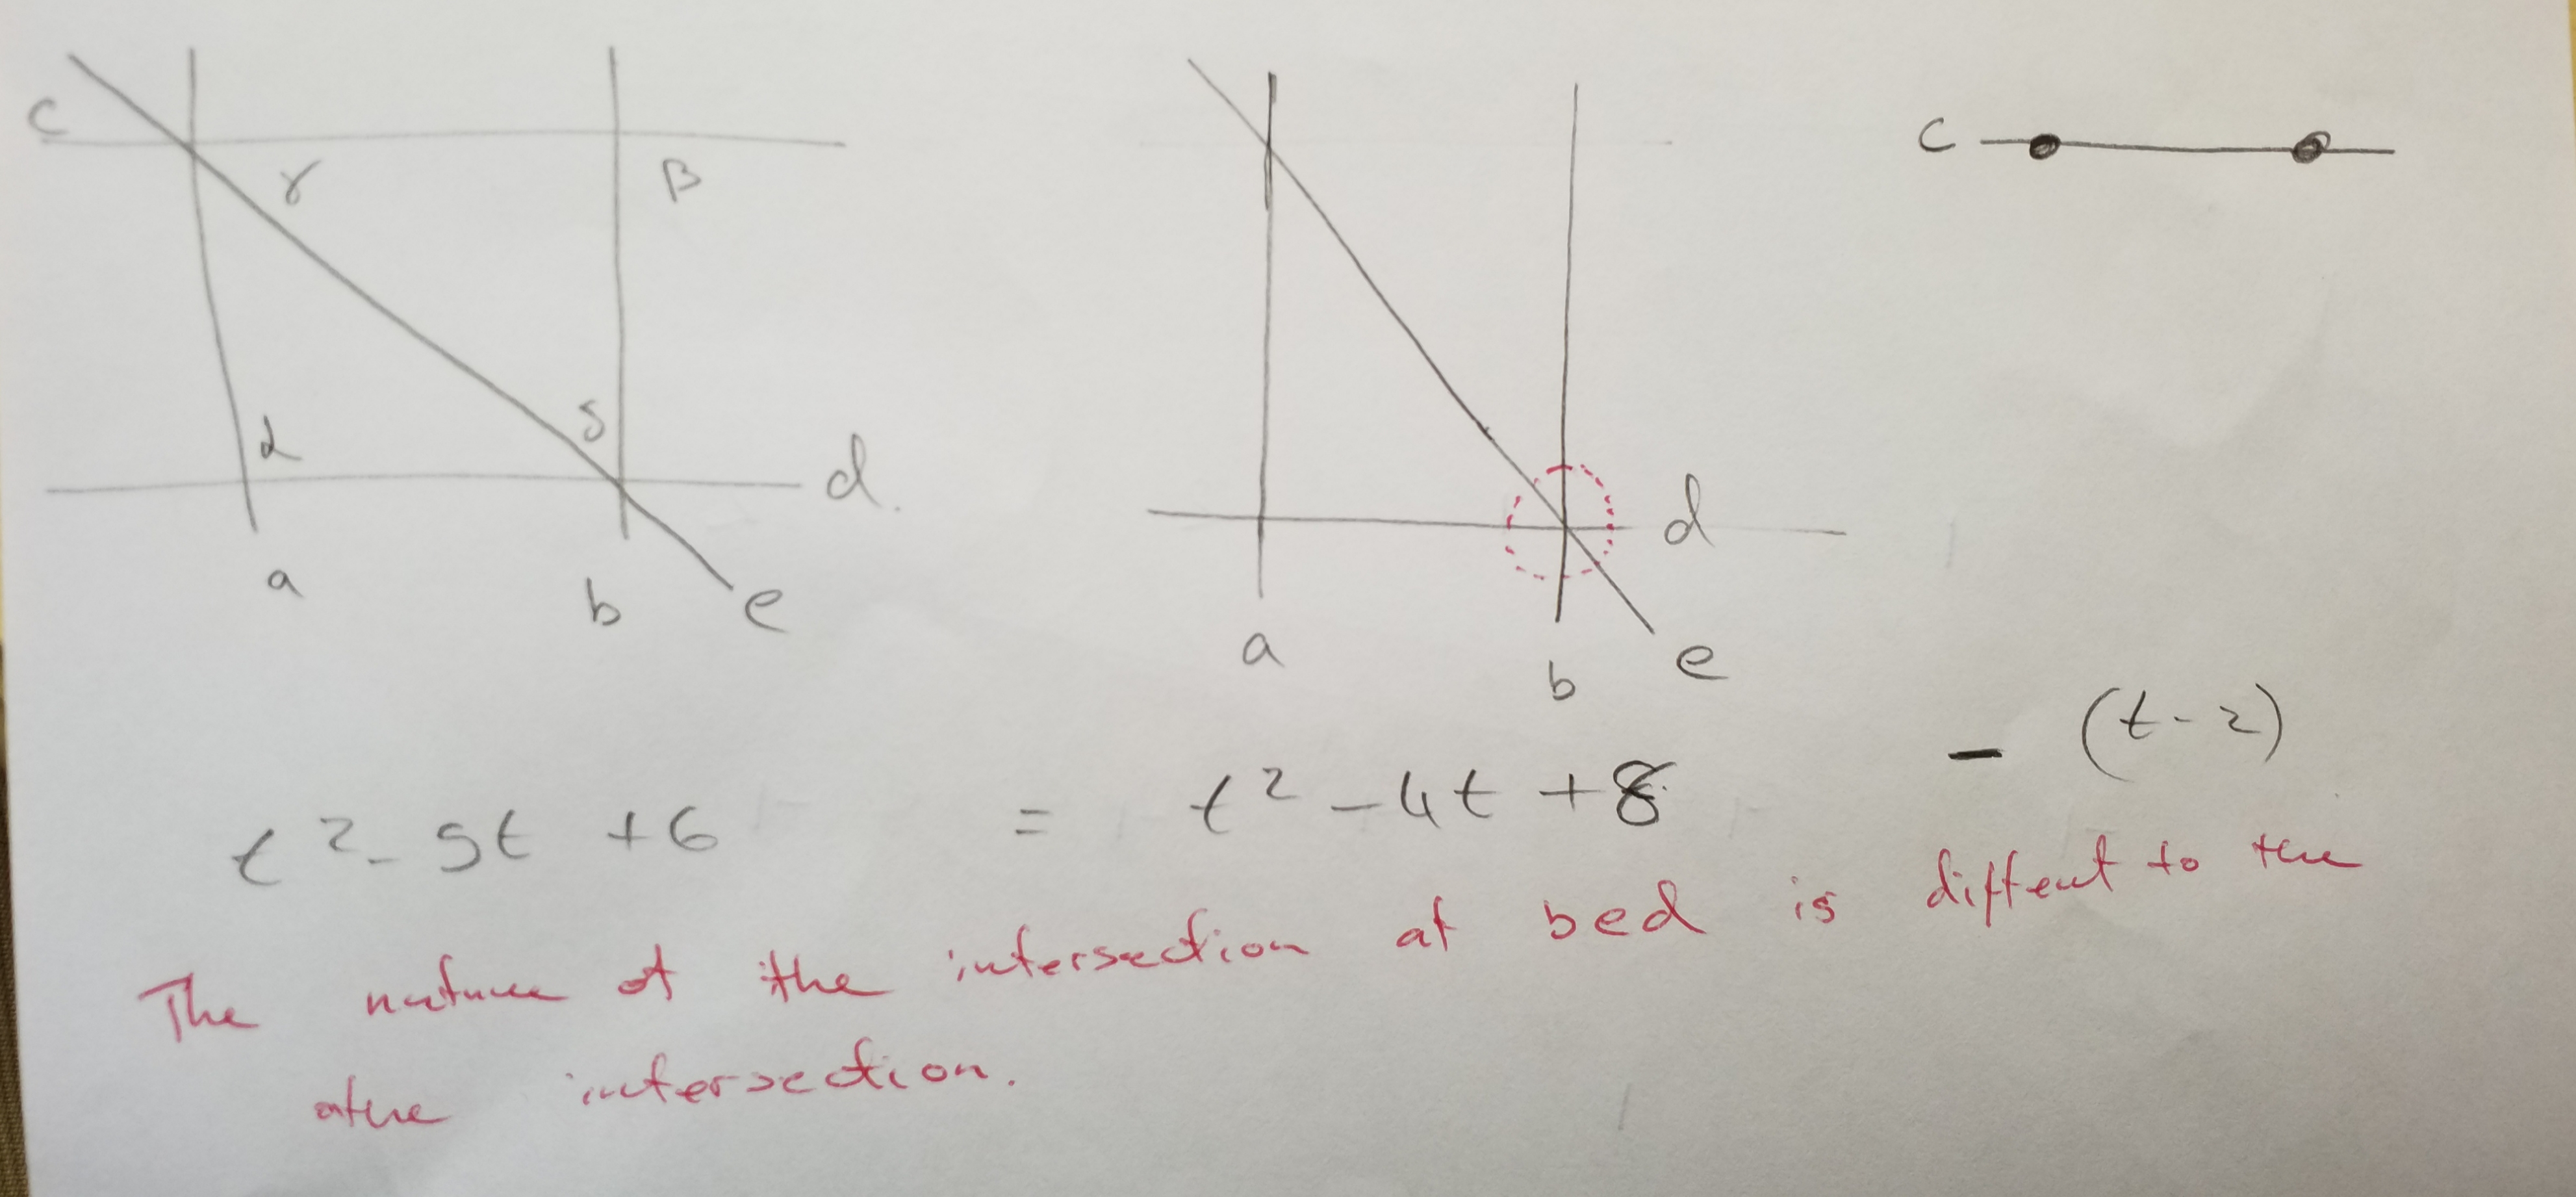
\includegraphics[scale=0.10,angle=0]{29072020 pics/del res qus.jpg}  
    \caption{Deletion-restriction of Figure 1 with a different choice of $H$}
    \label{poset}
\end{figure}

\item 
\begin{theorem}{(Cross-Cut theorem)} Let $x \in L(\mathcal{A})$ then 

$$\mu(x) =\sum_{\substack{\mathcal{B} \subseteq \mathcal{A} \\ \cap_{H\in \mathcal{B} } H = x}}  (-1)^{\# \mathcal{B}}. $

Previously, using the Möbius definition we needed to Möbius values for all intersections $z$ with $z \le x$. Now only need the hyperplanes that give $x$ and arrangeents $\mathcal{B}$.  

\end{theorem}

\begin{example}
\begin{figure}[H]
    \centering
 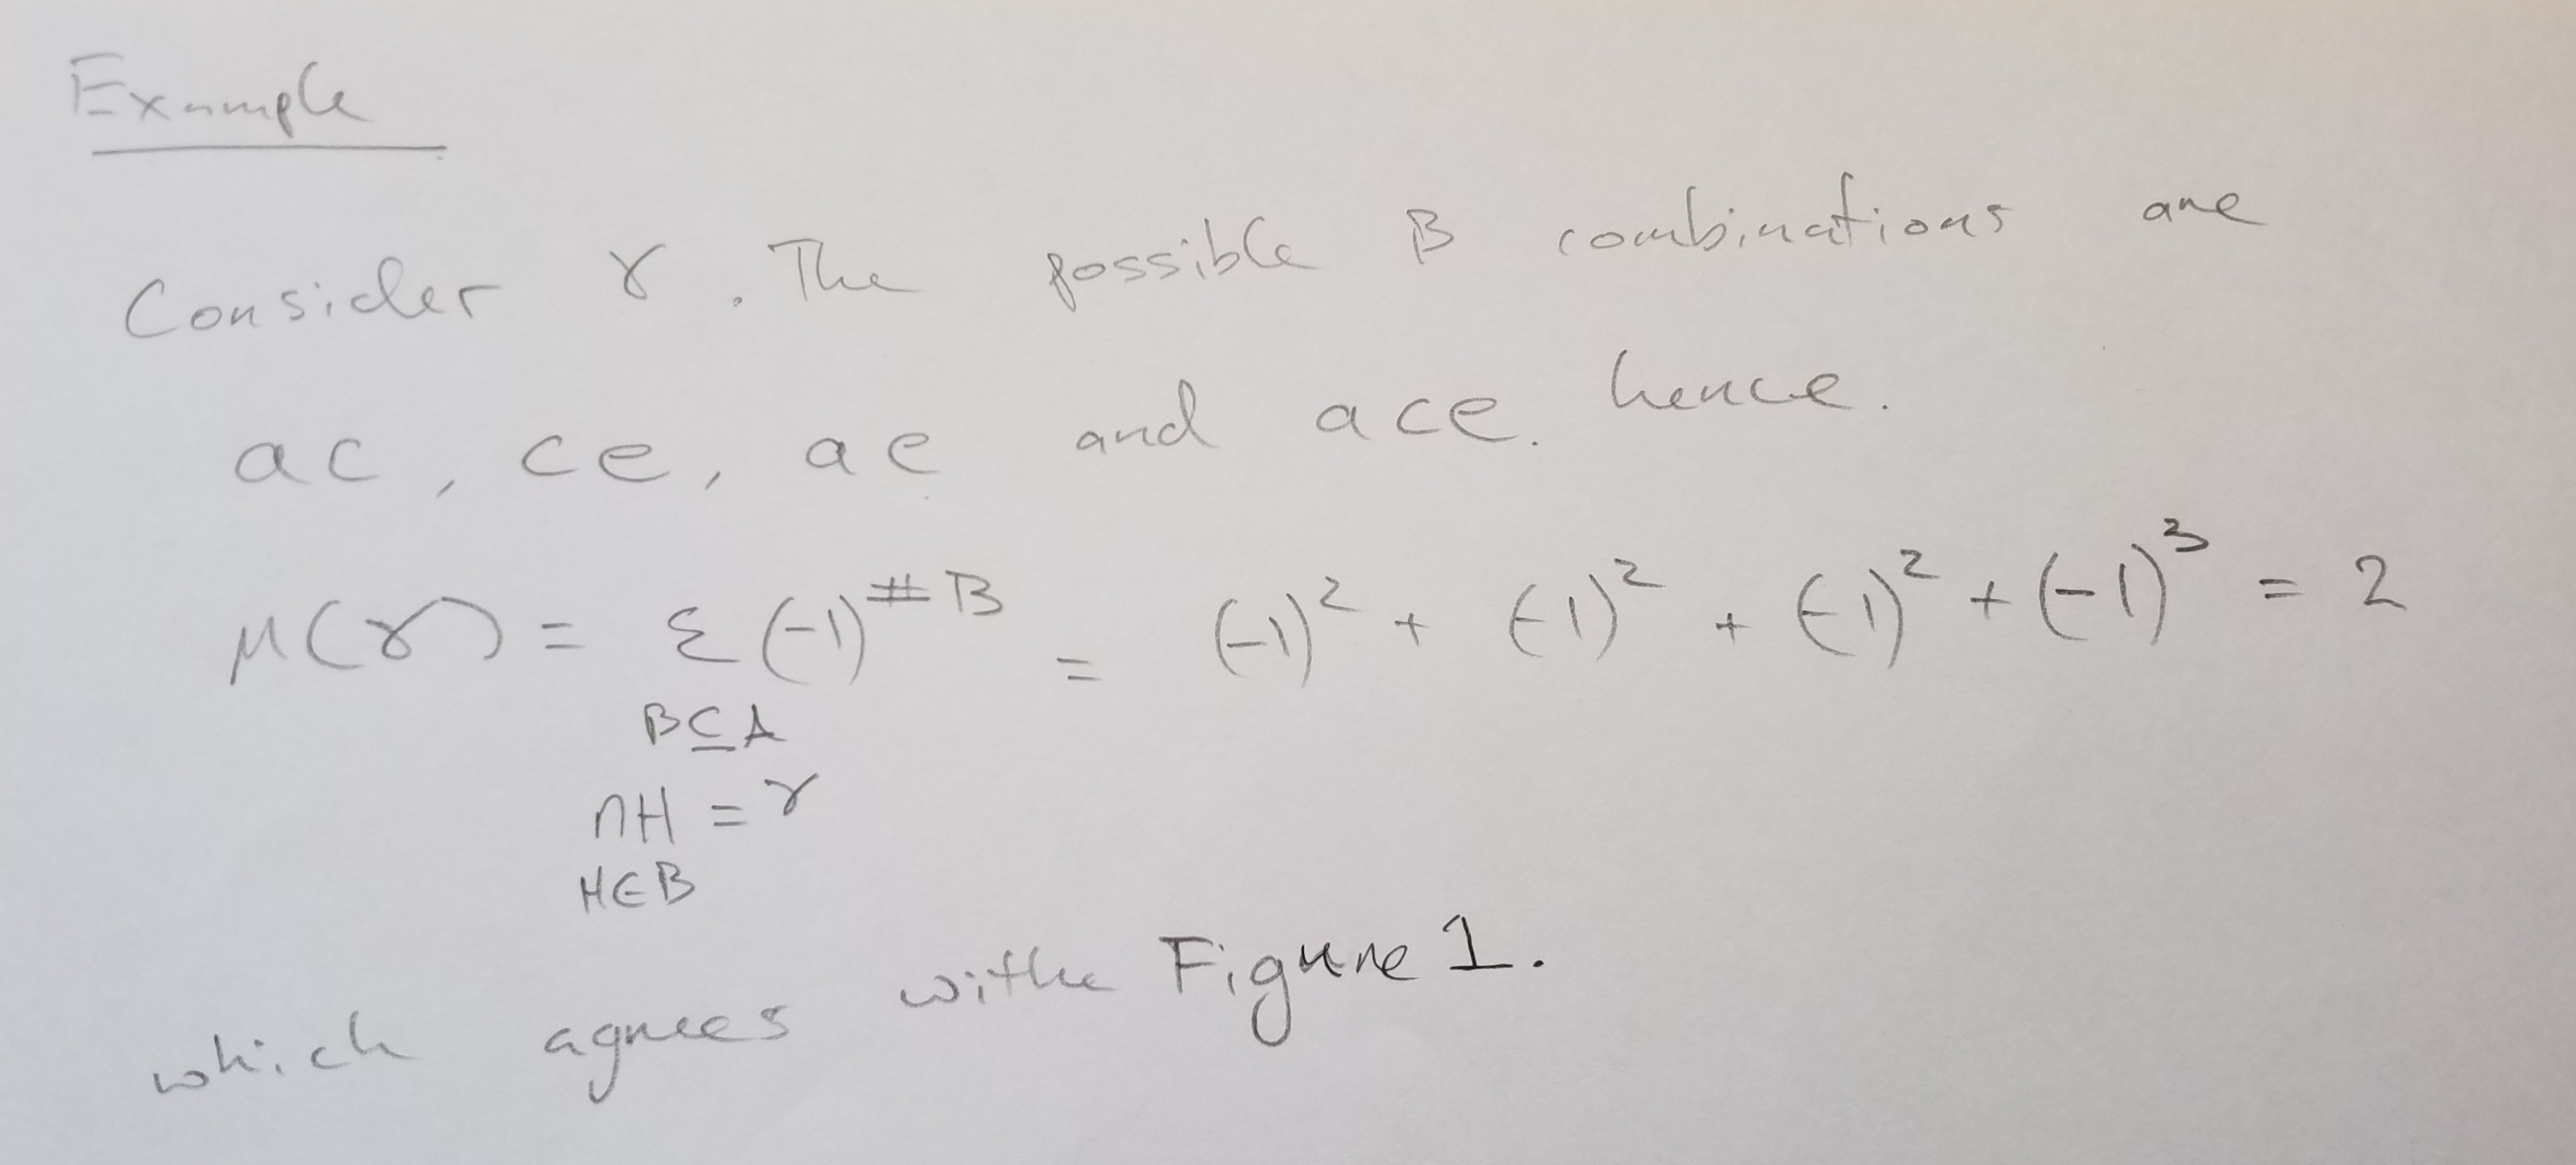
\includegraphics[scale=0.10,angle=0]{29072020 pics/cross cut.jpg}  
    \caption{Finding Möbius values using Cross-Cut theorem.}
    \label{poset2}
\end{figure}

\end{example}

\item \begin{example}\label{whitneythmapp}{Example of intersection poset with mobius values and with non-generic line in $\mathbb{R}^3$, using the Cross-Cut theorem.}



\begin{figure}[H]
    \centering
 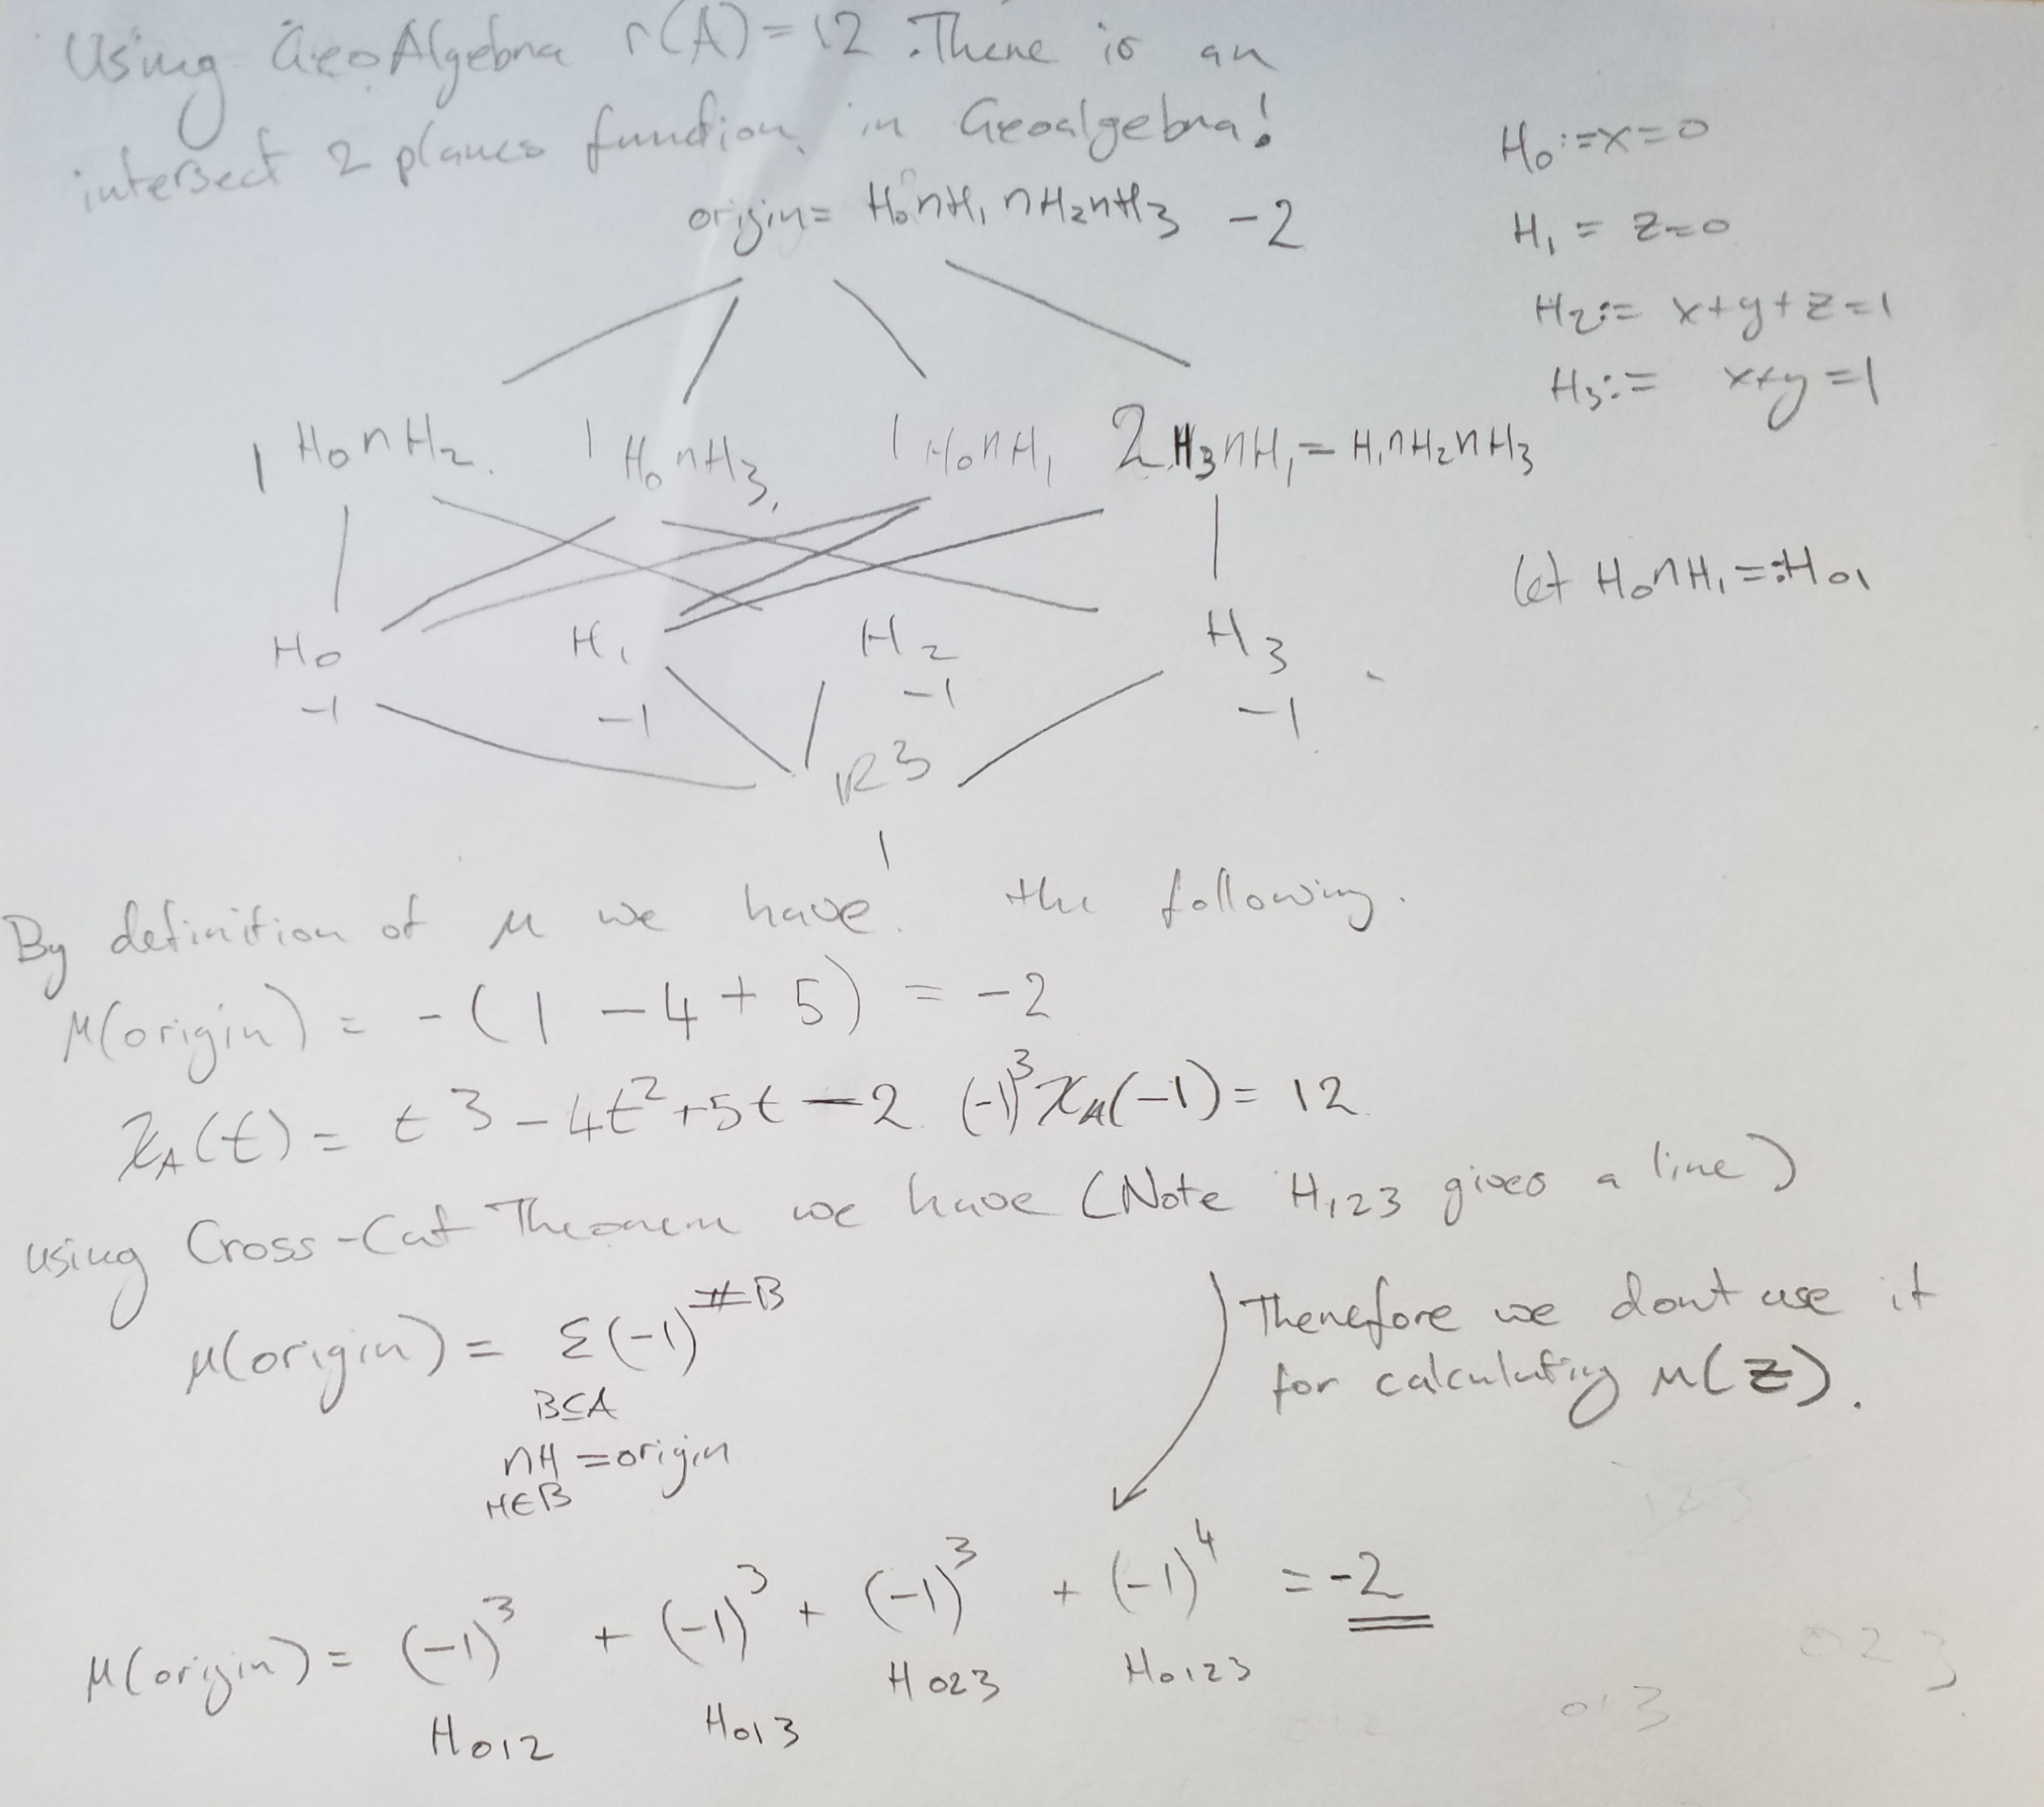
\includegraphics[scale=0.15,angle=0]{29072020 pics/R3 PosetExamp.jpg}  
    \caption{Using Cross-Cut in $\mathbb{R}^3$ non-generic situation}
    \label{poset3}
\end{figure}

\begin{figure}[H]
    \centering
 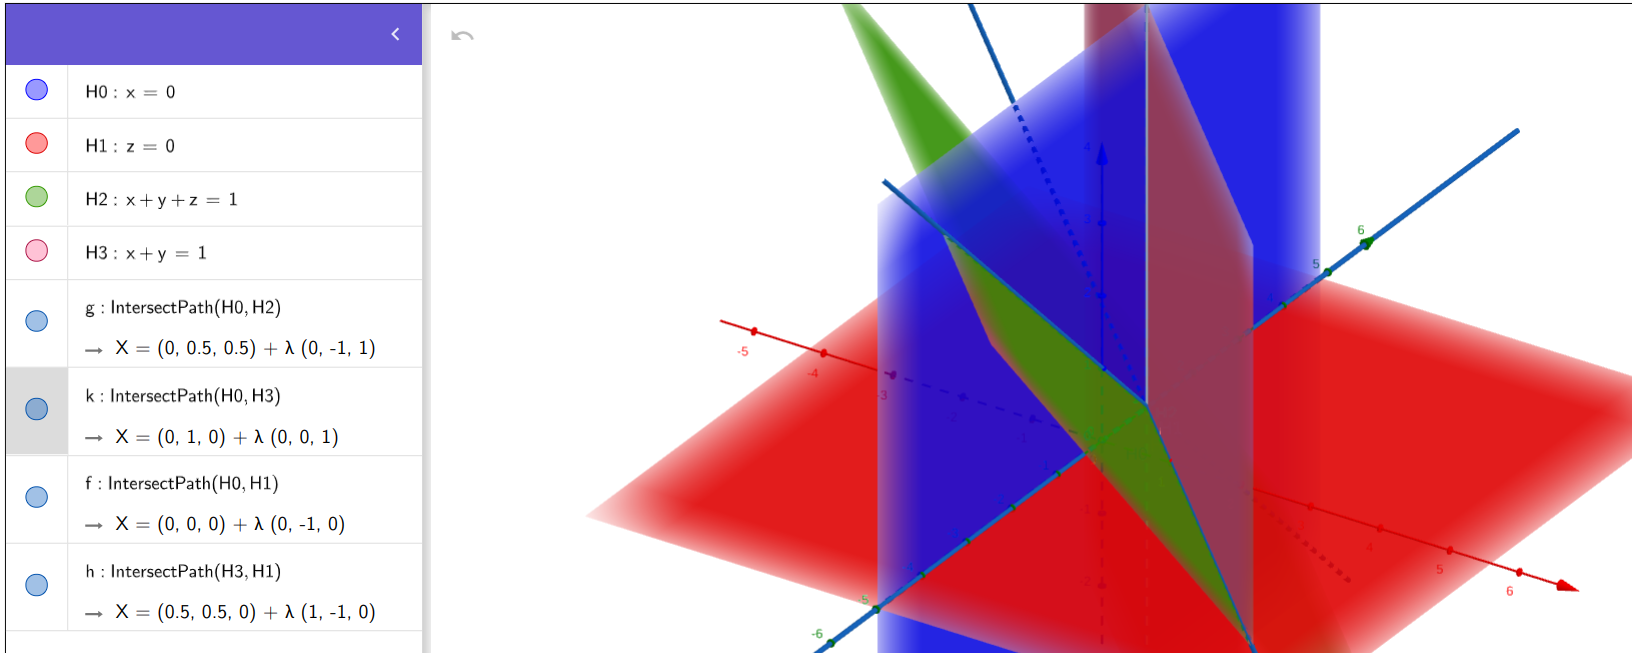
\includegraphics[scale=0.15,angle=0]{29072020 pics/Screenshot 2020-08-17 at 15.51.27.png}  
    \caption{The arrangement in $\mathbb{R}^3$}
\end{figure}

 
 \begin{remark}
    Recall example \ref{whitneythmapp}. There is a temptation to use Whitneys theorem to calculate $\mu(pt)$. In that case we noted that $H_{123}$ gave a line. Determining which $\mathcal{B}\subset \mathcal{A}$ gives a point is lengthy.
 \end{remark}
 
 \item  \subsection{SAGE & toric arranmgnet}

Investigate the SAGE code in \cite{ChenTHEARRANGEMENTS}



\item \begin{figure}[htp]

\centering
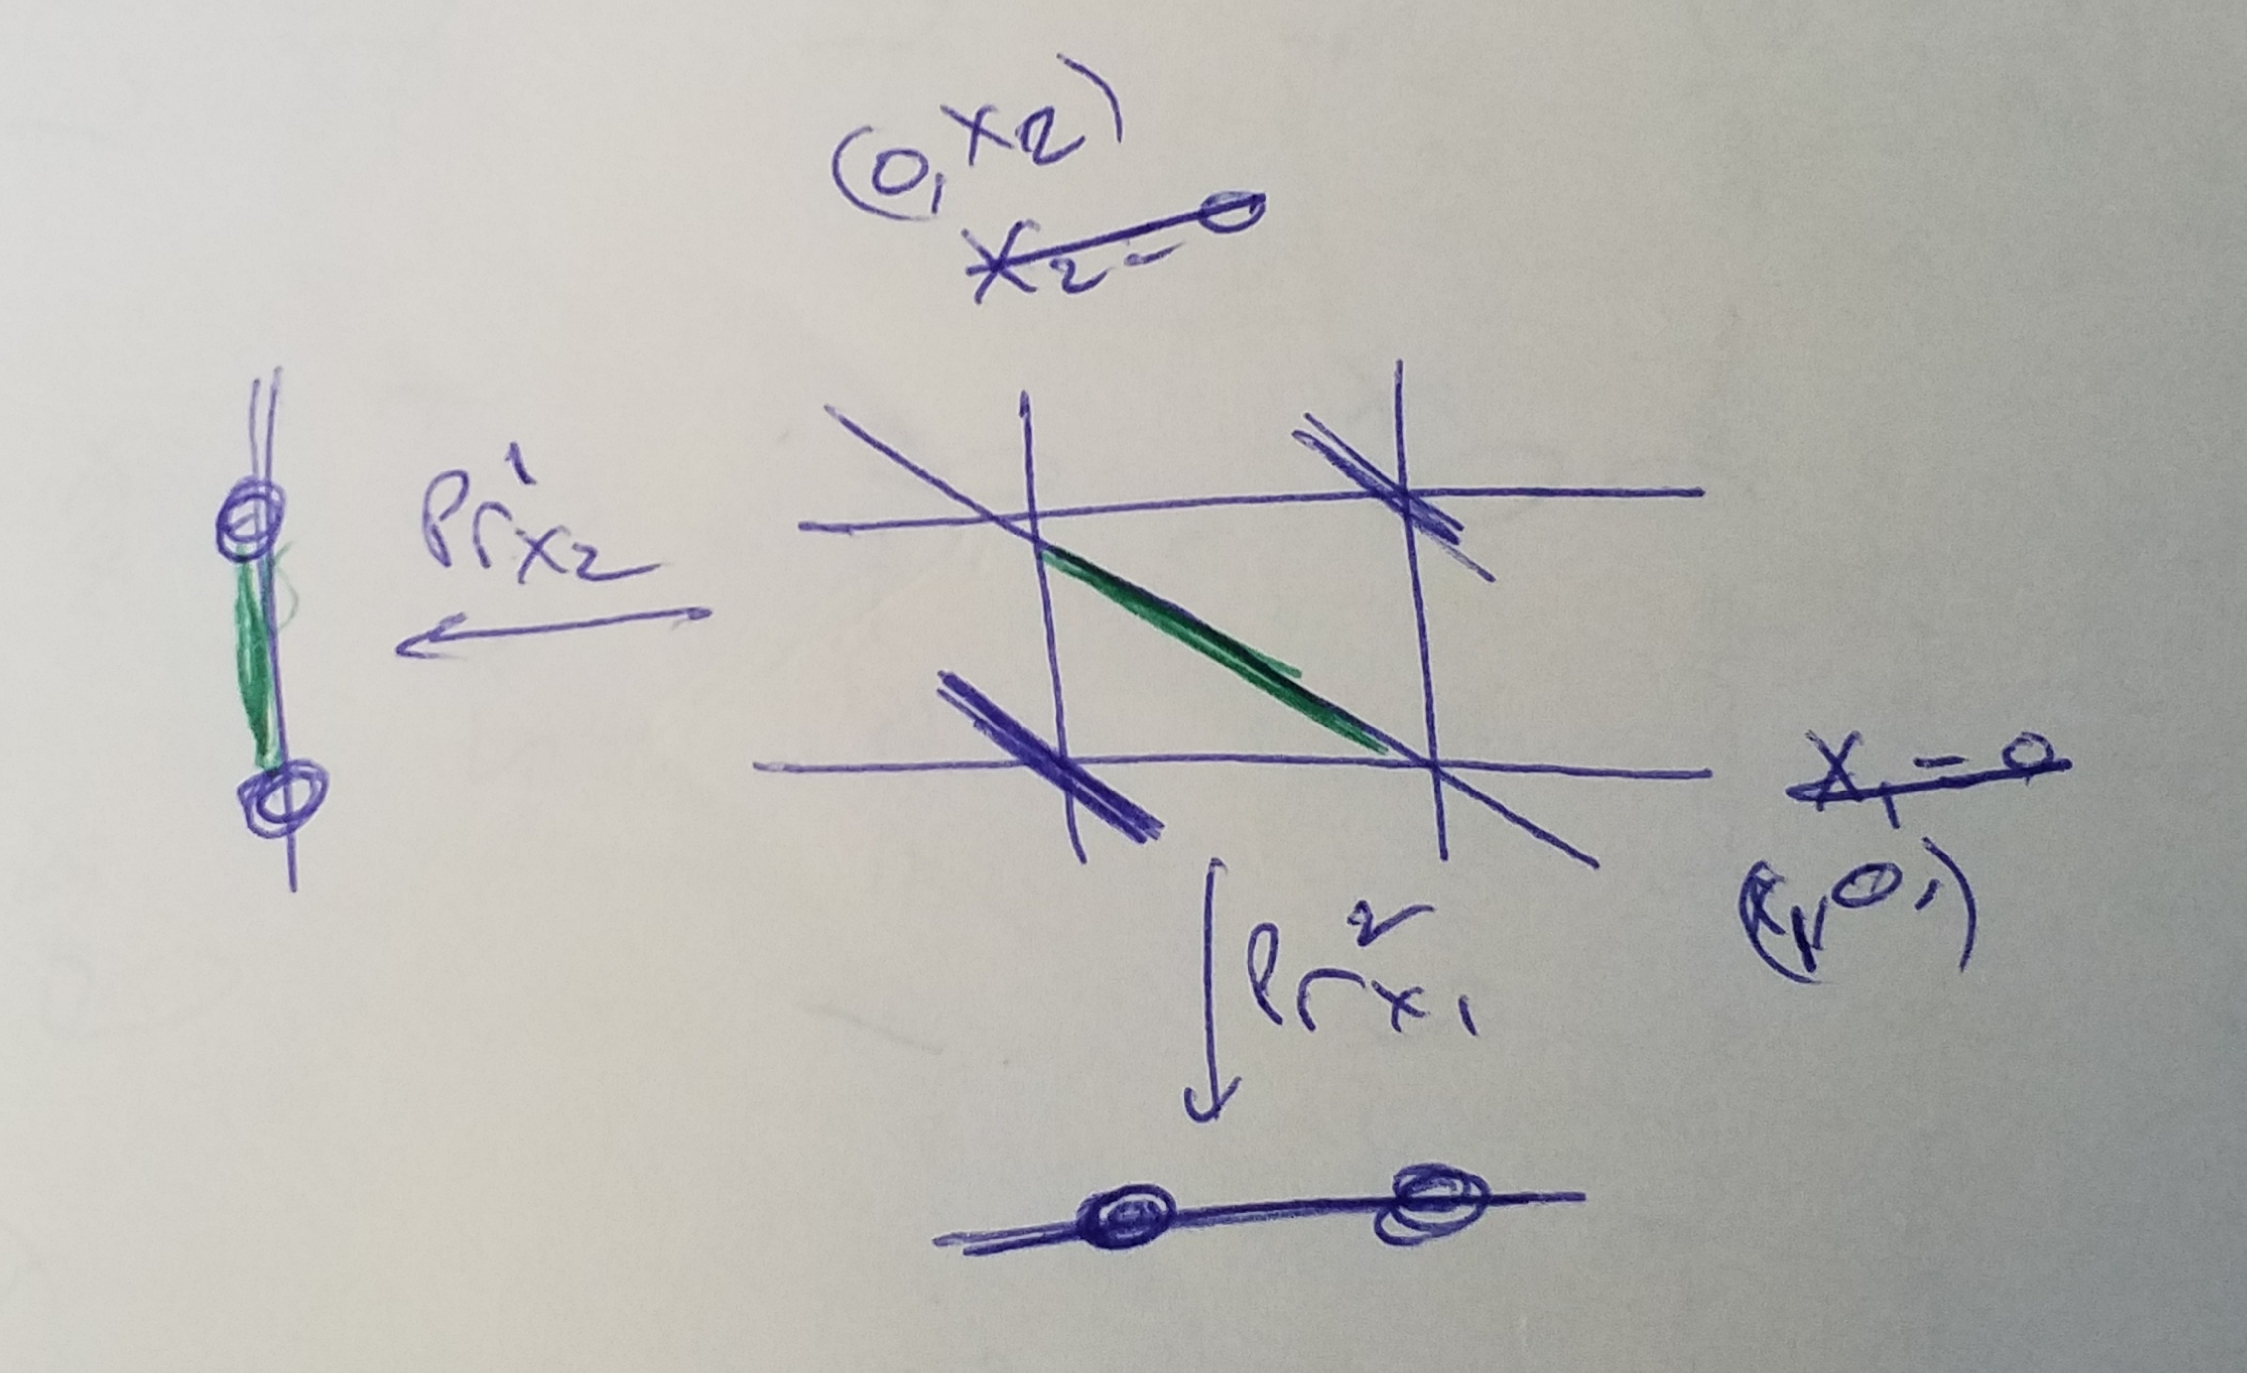
\includegraphics[width=.45\textwidth]{29072020 pics/PrjR2.jpg}\hfill
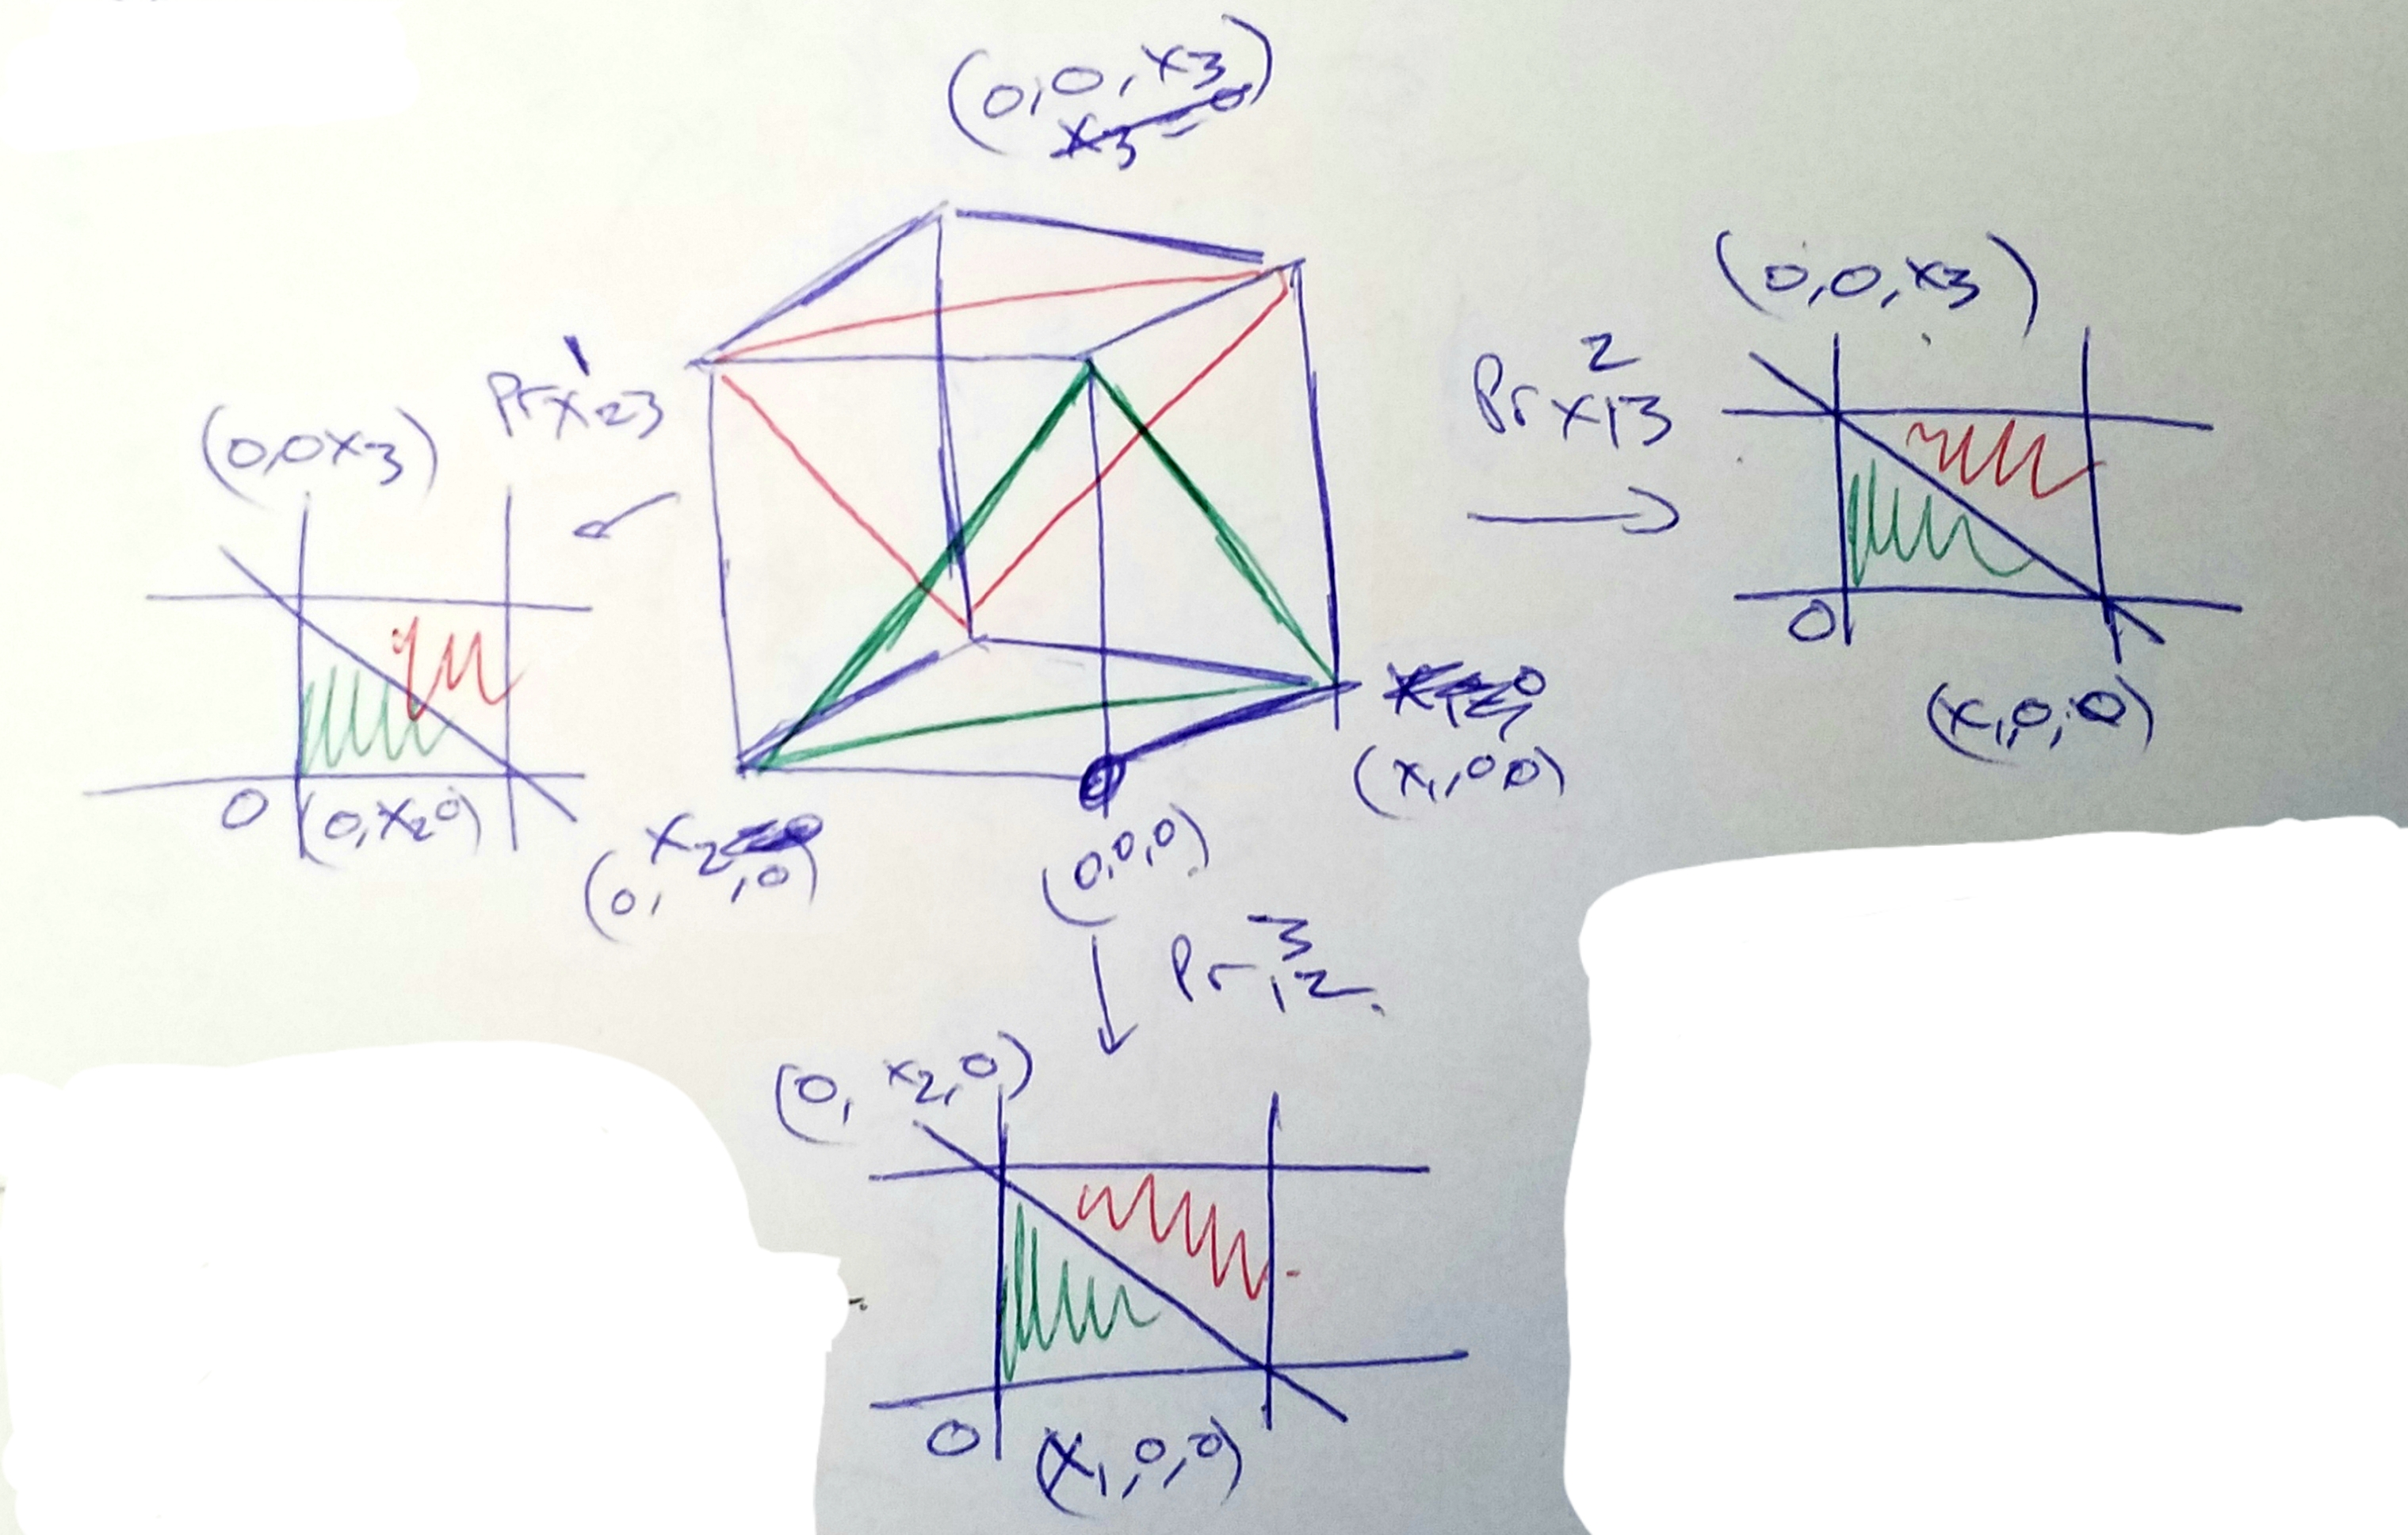
\includegraphics[width=.55\textwidth]{29072020 pics/prjR3.jpg}
\caption{Projection onto faces in $\mathbb{R}^2$ and $\mathbb{R}^3$.}
\label{}
\end{figure}

\item \begin{figure}[H]
\begin{center}
    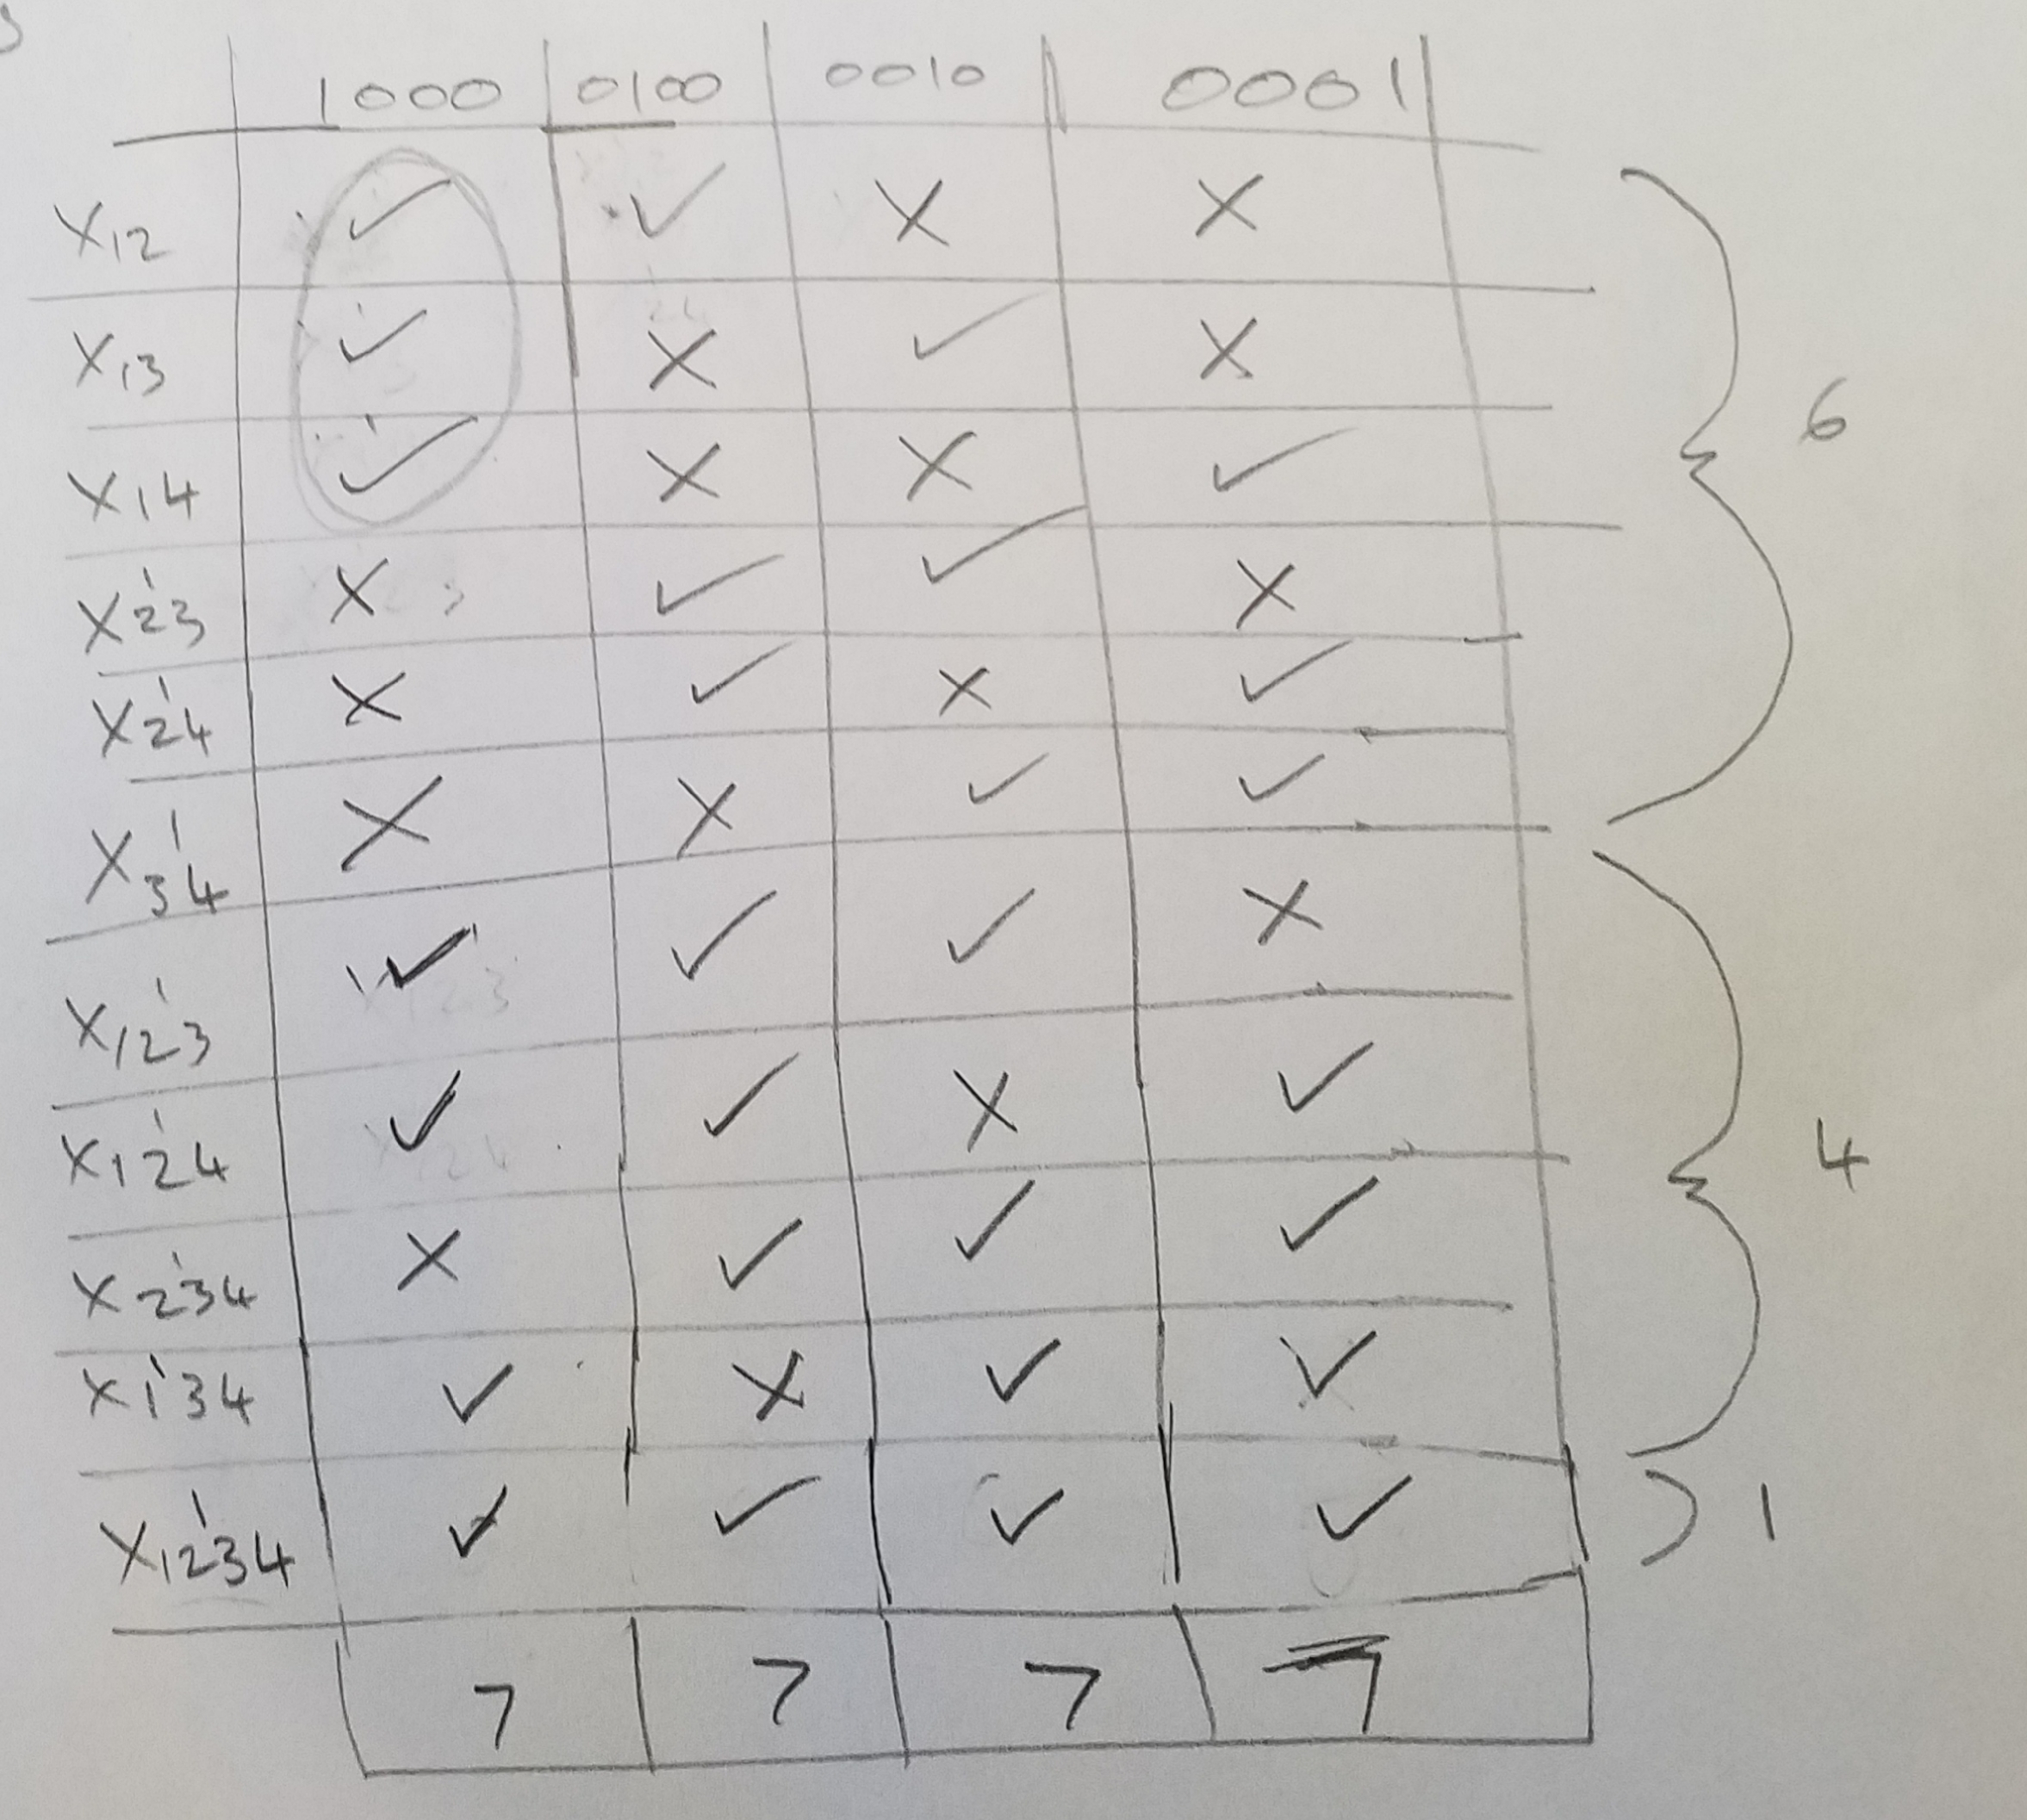
\includegraphics[width=.5\textwidth]{29072020 pics/fundpts.jpg}
\caption{Hyperlanes intersecting $x_{i}^0$ and at which points}
\label{}
\end{center}
\end{figure}

\item  
 \subsection{Attempt (In progress): Counting regions in $\mathbb{R}^4$}

Consider the $\mathbb{R}^3$ case. Take $(\frac{1}{2},\frac{1}{2},\frac{1}{2})$, we have $x_{ij}^1$ consider the intersection with $x_1^0$ on $x_{12}^1$ have $(0,1,-)$, where $-$ is a free variable (orthogonal projection), and similarly on $x_{13}^1$ have $(0,-,1)$ on $x_{23}^1$ this gives the line $x_{23}^1$. Similarly for $x_2 =x_3 =0$

\begin{figure}[H]
    \centering
    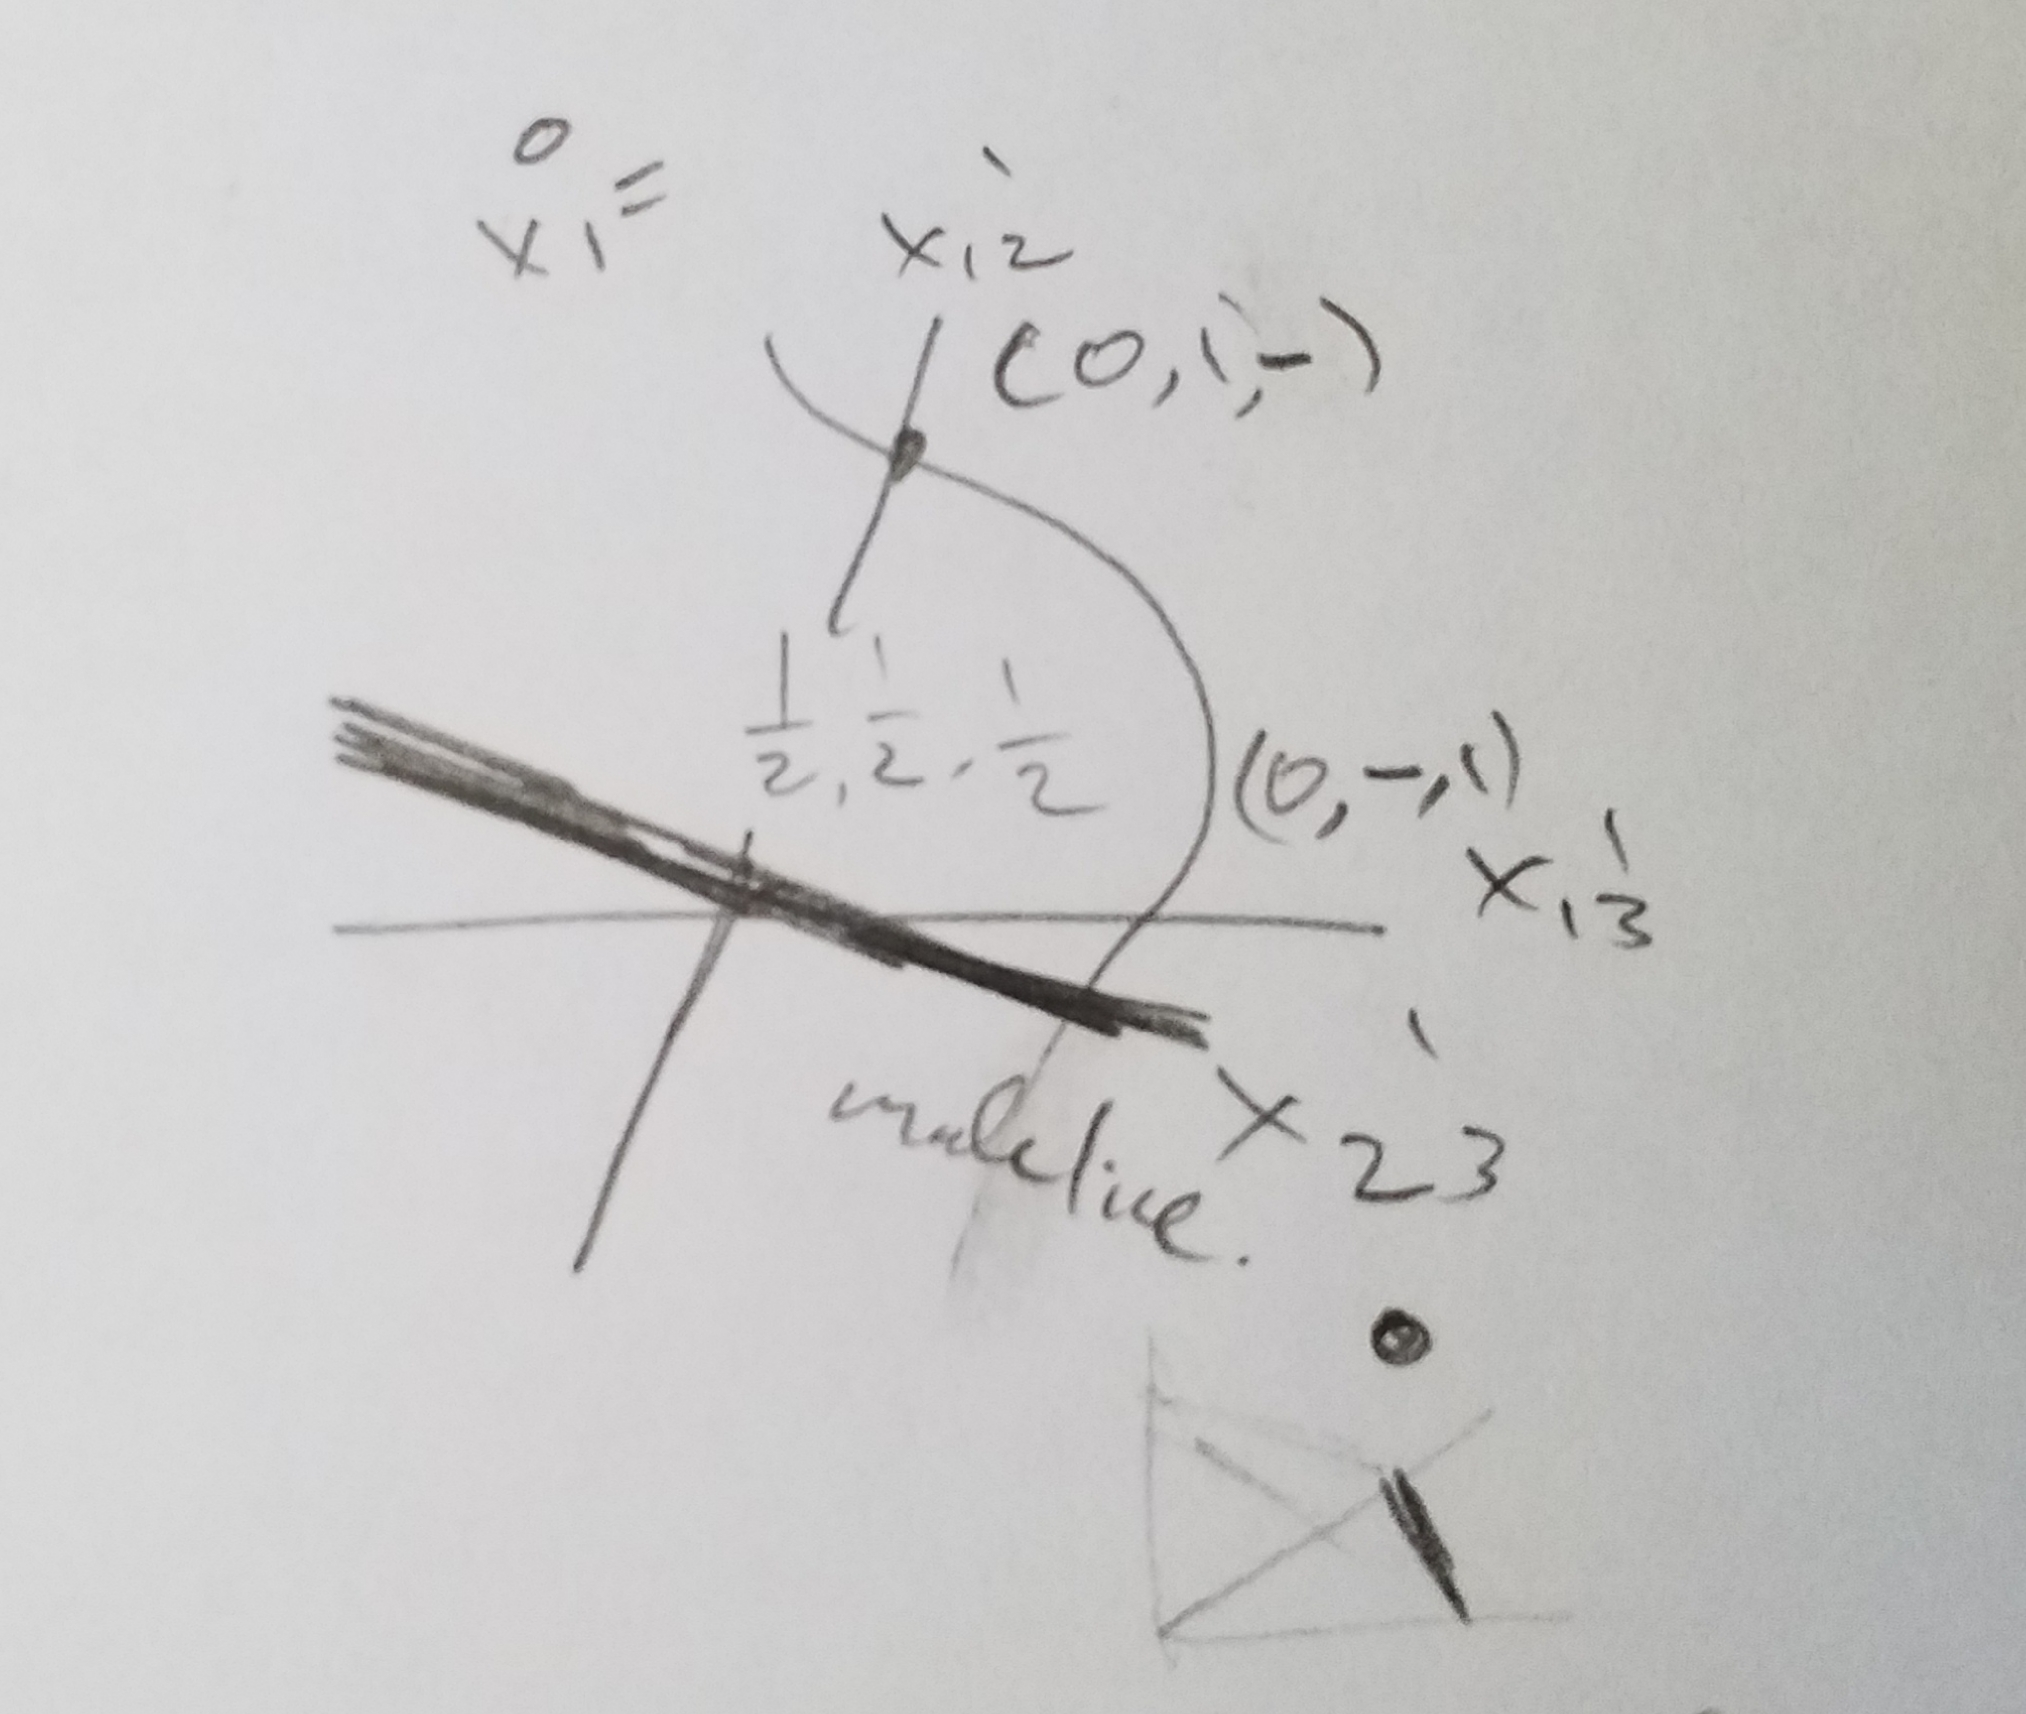
\includegraphics[width=.5\textwidth]{29072020 pics/point12R2.jpg}
    \caption{Caption}
    \label{fig:my_label}
\end{figure}


Consider the $\mathbb{R}^4$ case (with only these hyperplanes) take $(\frac{1}{3},\frac{1}{3},\frac{1}{3},\frac{1}{3})$ the intersection of $x_{ijk}^1$ (total of 4 hyperplanes), giving 16 regions.

\begin{figure}[H]
    \centering
    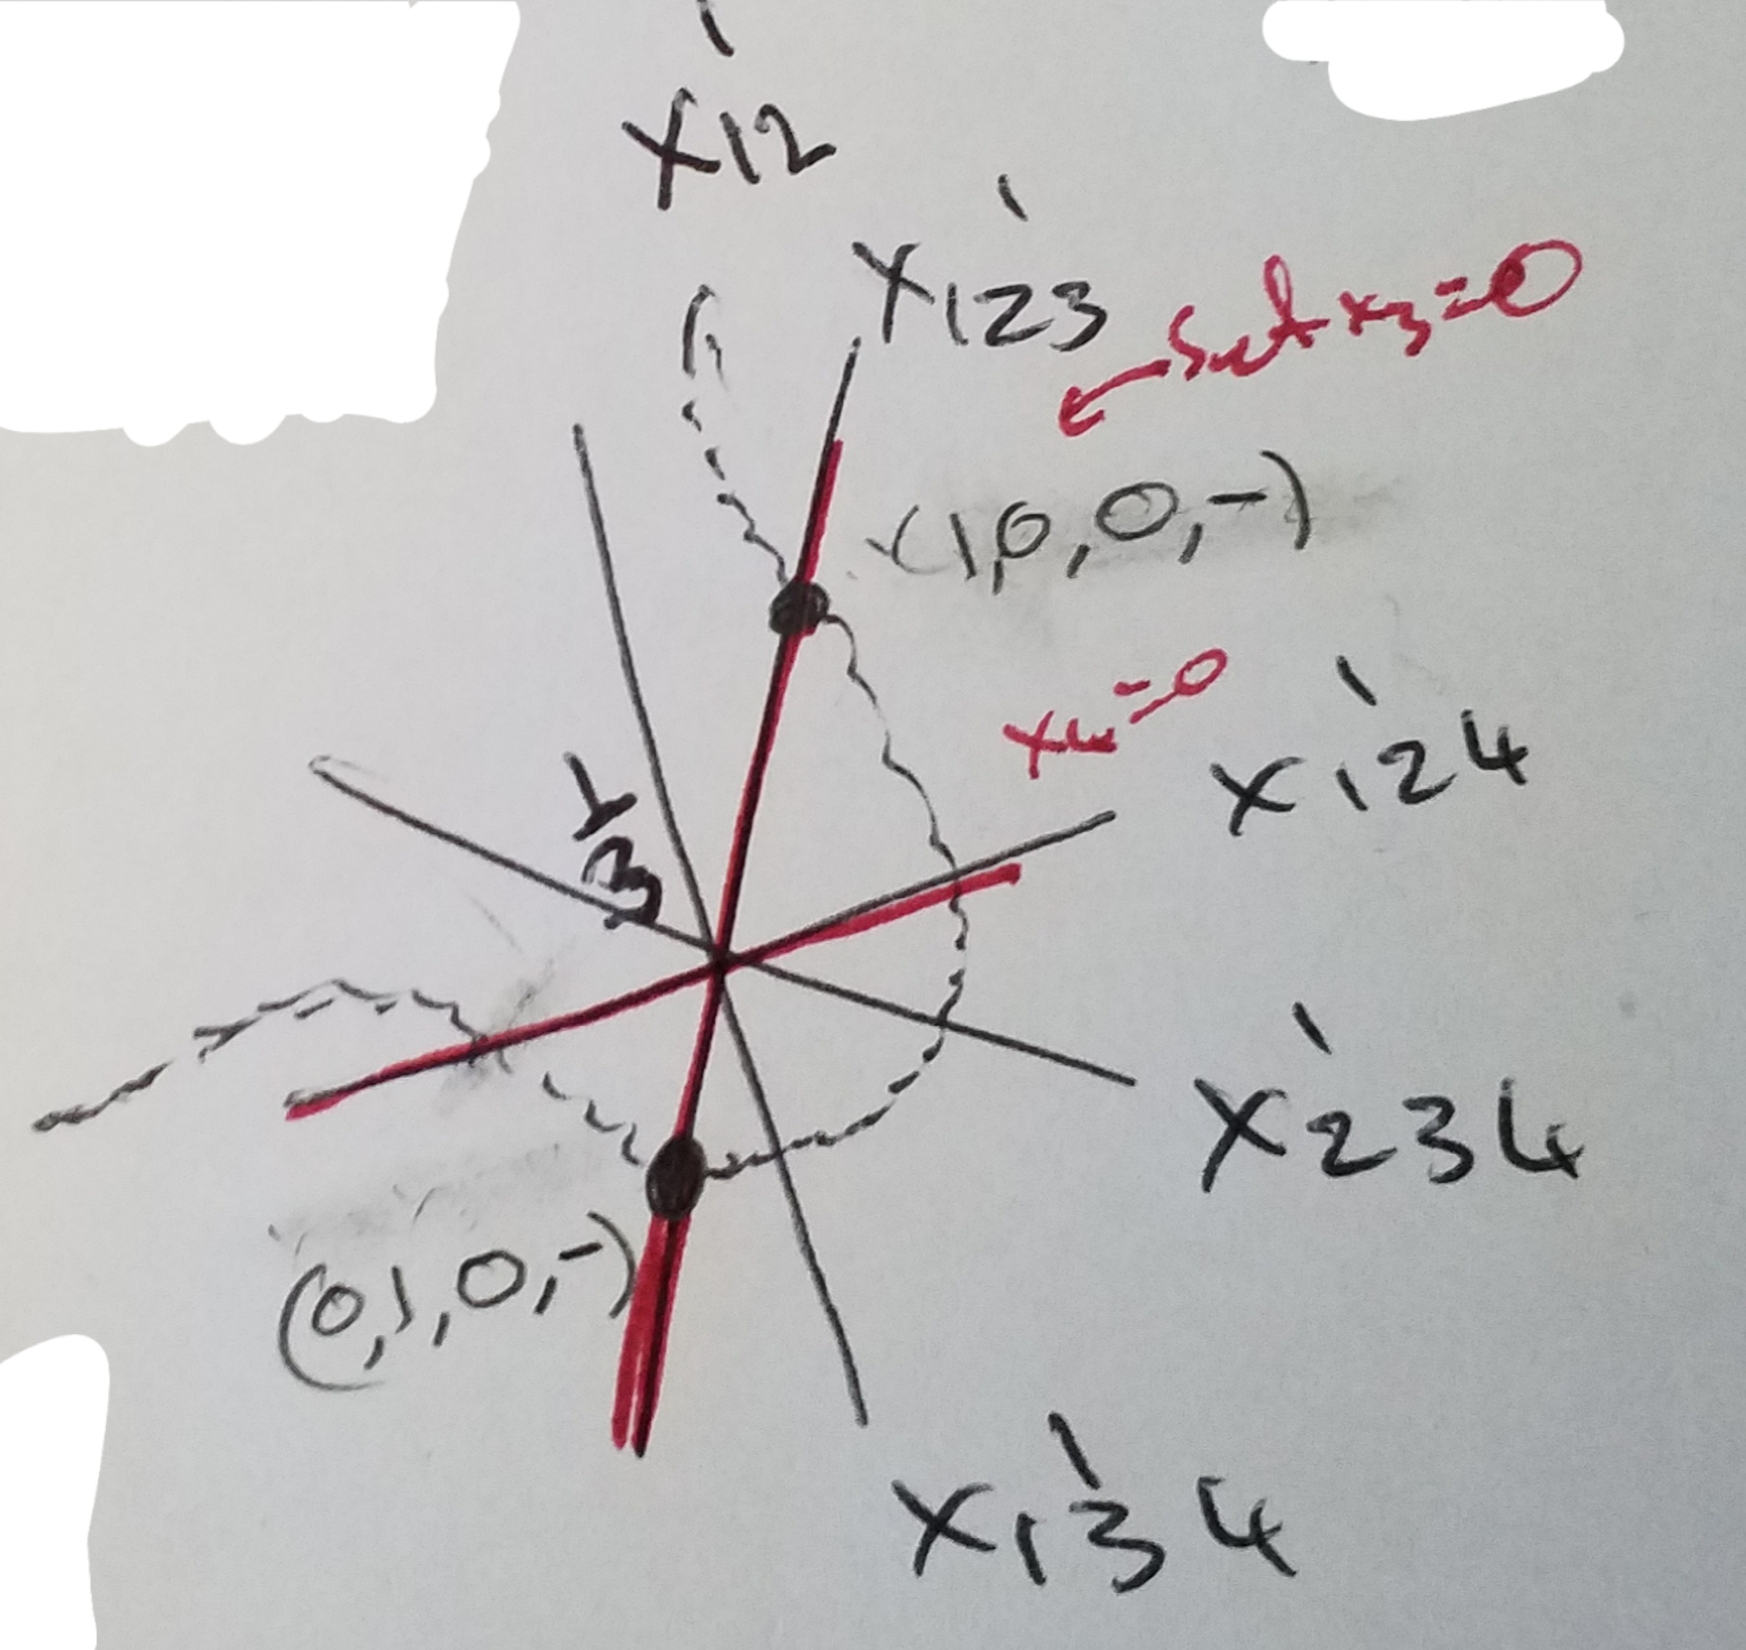
\includegraphics[width=.5\textwidth]{29072020 pics/point13r4.jpg}
    \caption{Caption}
    \label{fig:my_label}
\end{figure}


Add the hyperplane $x_{12}^1$ into this arrangment, then $x_{234}^1$ and $x_{134}^1$ are cut in half, and $x_{123}^1$ and $x_{124}^1$ are not (why: redundancy: equation sits inside the other). Considering all hyerplanes of type 2 we get $16+4*6=40$. 



If we can show also show that $x_{1234}^1$ and $x_{1234}^3$ gives a region in each corner (0,0,0,0) and (1,1,1,1). 

We also have 40 regions at $(\frac{2}{3},\frac{2}{3},\frac{2}{3},\frac{2}{3})$

Now considering $(\frac{1}{2},\frac{1}{2},\frac{1}{2},\frac{1}{2})$ we have $x_{1234}^2$ and all 6 of type $x_{ij}^1$, where the $x_{ij}^1$ intersect generically (codminension argument question 6>4 the total dimension of the space, might not get $2^6$ ).assuming generically we get $2^6$ regions. Then all the redundancies lie in $x_{1234}^2$.

Then one has disjoint pairs, $x_{12}^1$ & $x_{34}^1$
$x_{13}^1$ & $x_{24}^1$
$x_{14}^1$ & $x_{23}^1$. For the other pairs on intersections one has for example $x_{12}^1$ & $x_{13}^1$ with $x_{1234}^2$, first we have $(1/2,1/2,-,-)$ from $x_{12}^1$, then forced to have $(1/2,1/2,1/2,-)$ for $x_{13}^1$, which forces  $(\frac{1}{2},\frac{1}{2},\frac{1}{2},\frac{1}{2})$ for  $x_{1234}^2$. Like wise for other ovelaping pairs.

There are 3 disjoint pairs, 3 generic cuts $2^3=8$.

Total 154?
\item 
Inverse projection collapsing polytopes.



\item 


\begin{theorem} {(Whitney's theorem)} Let $\mathcal{A}$ be an arrangement in $\mathbb{R}^n$. Then 

$$\chi_{\mathcal{A}} (t) = \sum_{\substack{\mathcal{B} \subset \mathcal{A}\\
\mathcal{B} \:\text{central}}}  (-1)^{\#\mathcal{B}} t ^{n-\text{rank}(\mathcal{B}) } .$$

\end{theorem}

\begin{example}
\begin{figure}[H]
    \centering
 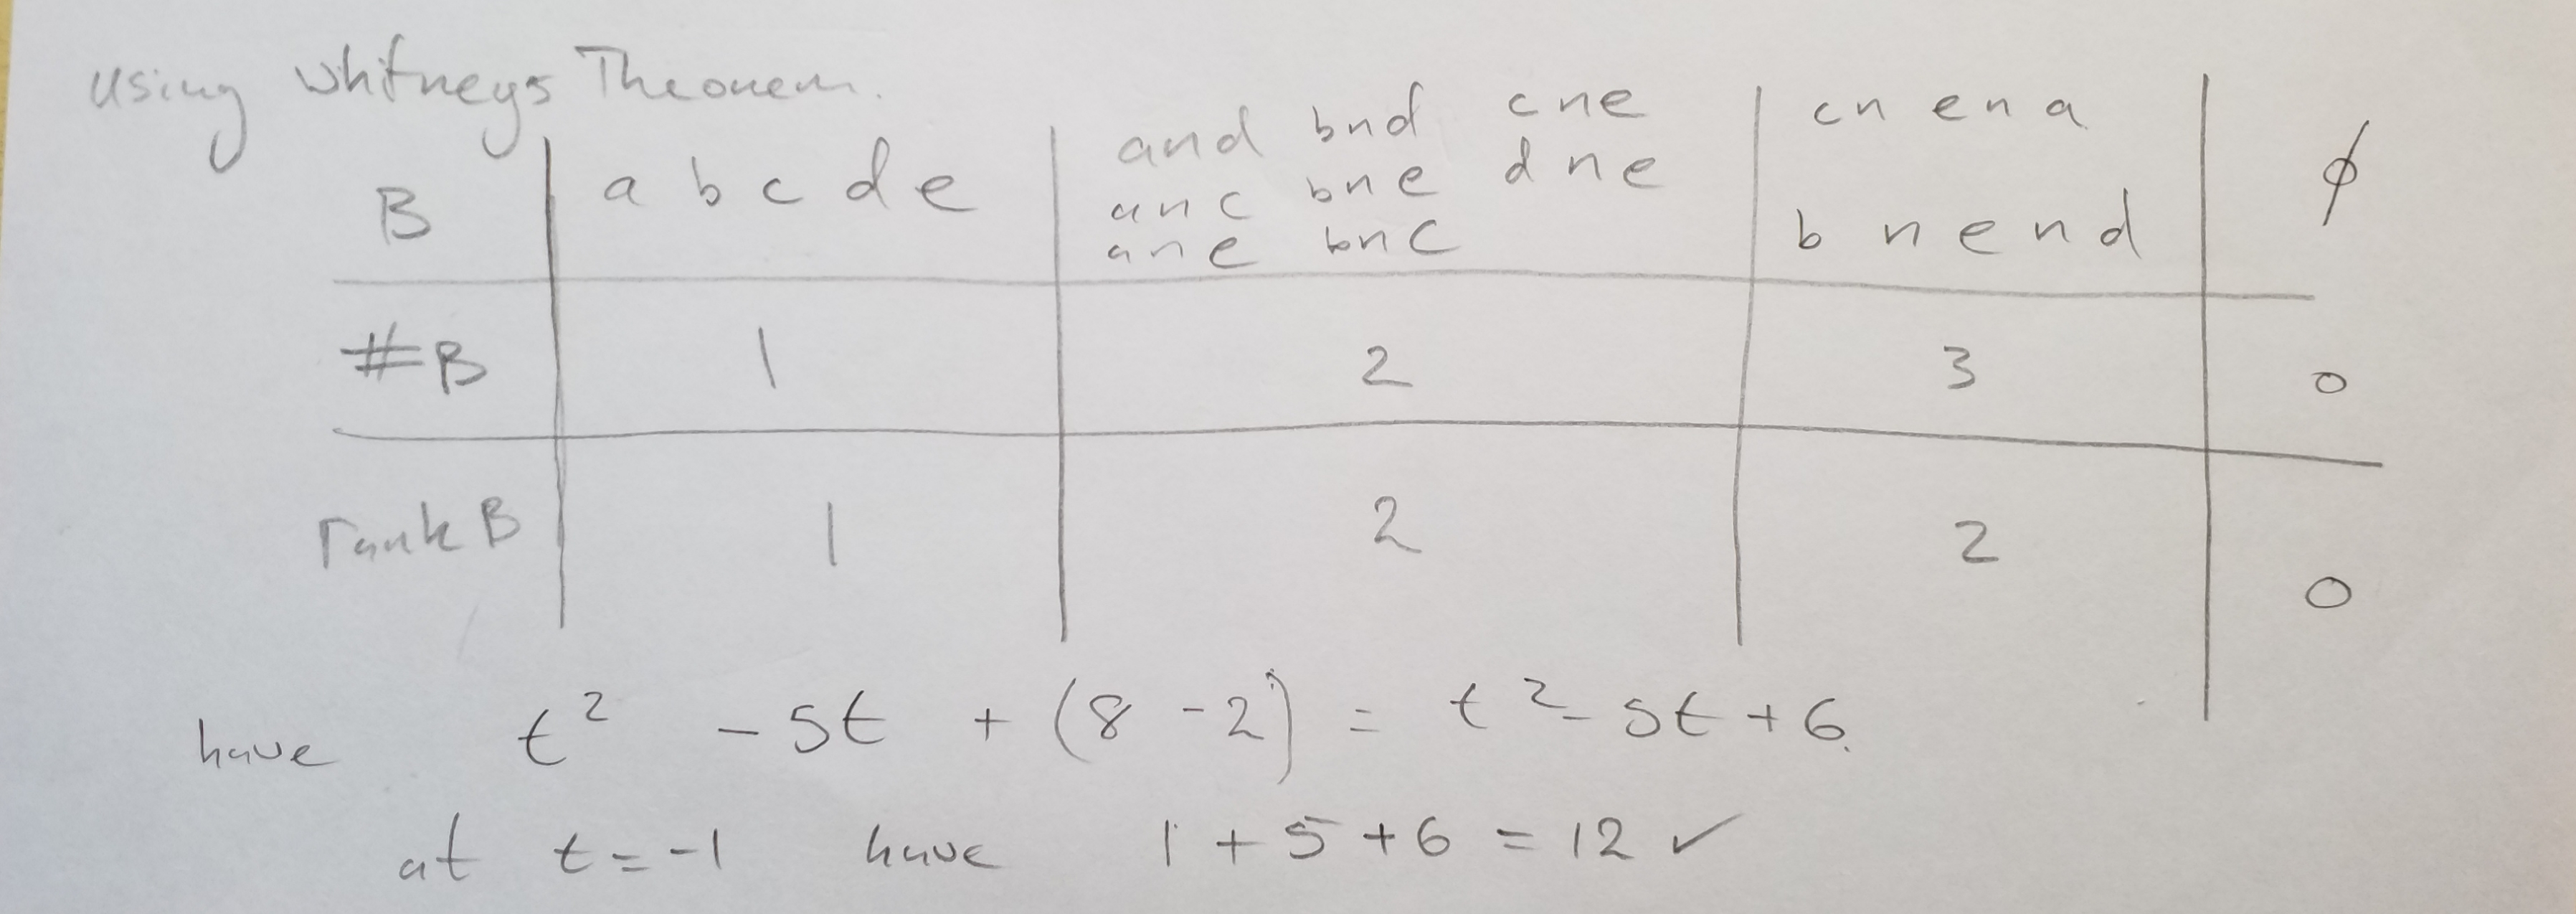
\includegraphics[scale=0.10,angle=0]{29072020 pics/whitney examp.jpg}  
    \caption{Determining the Möbius value only using hyperplanes, $\mathbb{R}^2$ case}
    \label{poset}
\end{figure}

\end{example}

\end{example}

\end{titlemize}






\printindex

\bibliographystyle{alpha}
\bibliography{bibtex}





\end{document}
